\documentclass[aspectratio=169]{beamer}
\usetheme{Madrid}

\usepackage{tikz}
\usepackage{url}

\title{Intro to \LaTeX}
\author{Andrew Huang}

\institute[University of Melbourne]

\titlegraphic{
	
\includegraphics[height=0.1\linewidth]{./Images/mueec_logo.png}
	\hspace{2.5cm}
	
\includegraphics[height=0.1\linewidth]{./Images/arrp_logo.png}
}

\AtBeginSection[]
{
	\begin{frame}<beamer>{Outline}
		\tableofcontents[currentsection,currentsubsection]
	\end{frame}
}

\newcommand\blfootnote[1]{%
	\begingroup
	\renewcommand\thefootnote{}\footnote{#1}%
	\addtocounter{footnote}{-1}%
	\endgroup
}

\begin{document}
\begin{frame}
    \maketitle
\end{frame}

\begin{frame}{Outline}
	\tableofcontents
\end{frame}

\section{Why \LaTeX?}
\begin{frame}{\insertsection}
	\begin{figure}
		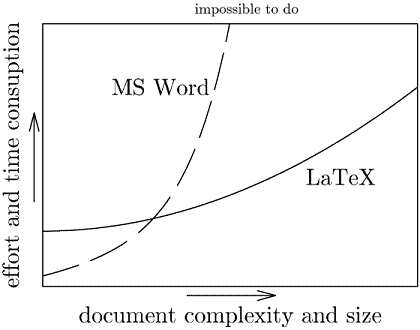
\includegraphics[scale=0.5]{./Images/latex-difficulty-2.png}
	\end{figure}
\end{frame}

\begin{frame}{\insertsection}{Work flow improvements}
	\begin{figure}
		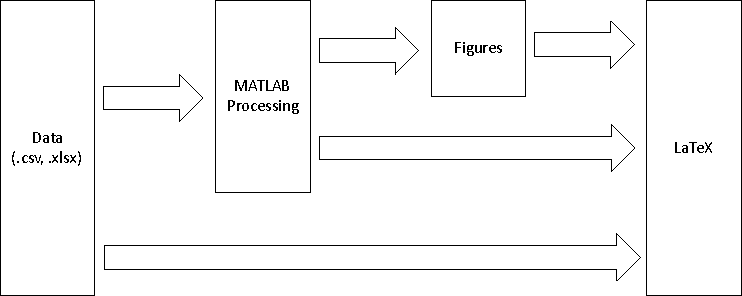
\includegraphics[width=0.7\linewidth]{./Images/workflow.pdf}
	\end{figure}
\end{frame}

\begin{frame}{\insertsection}{Pretty Pictures}
	\begin{figure}
		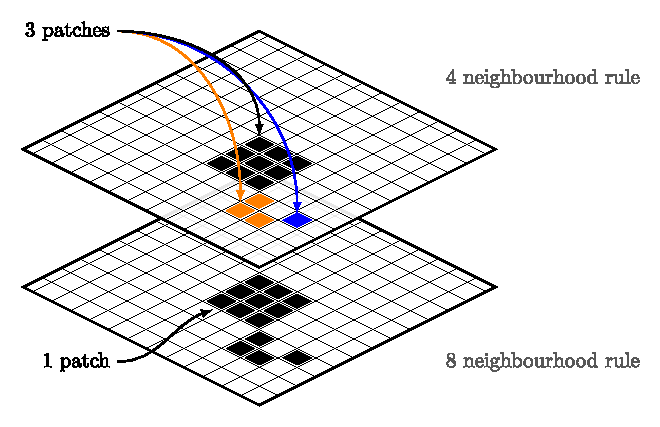
\includegraphics[width=0.35\linewidth]{./Images/Neighbourhood_definition2.pdf}
		\hspace{5em}
		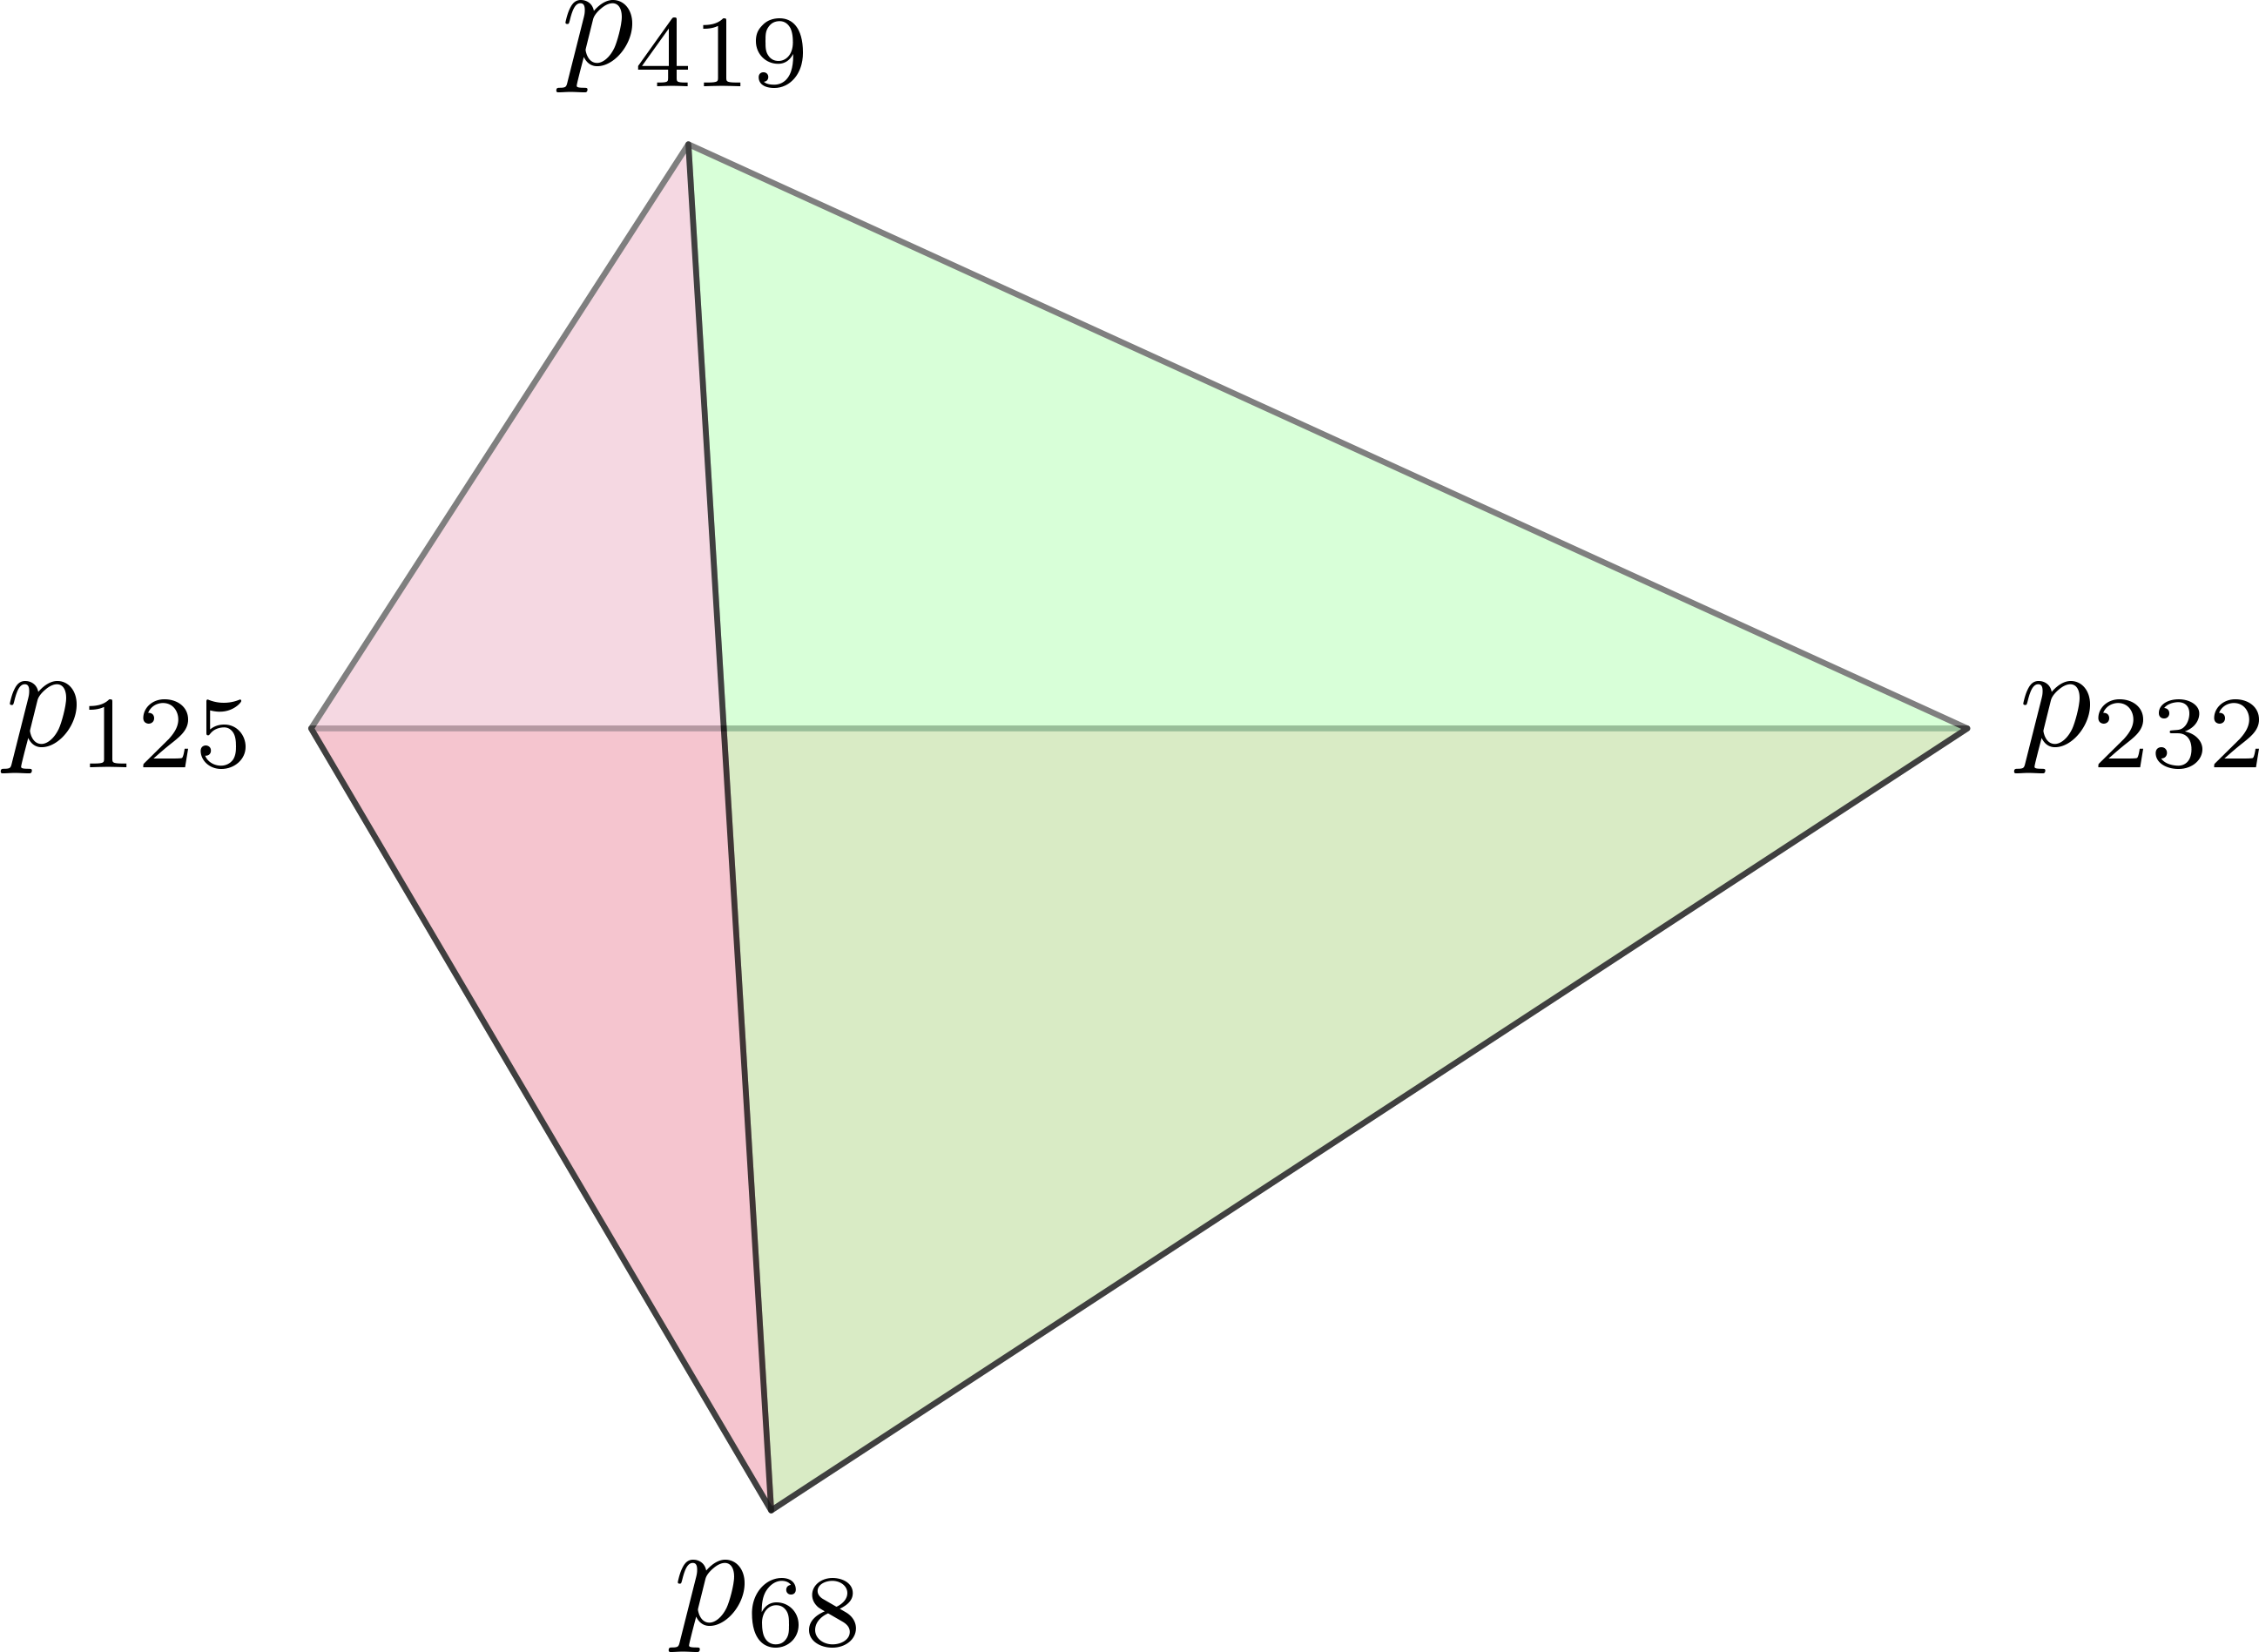
\includegraphics[width=0.35\linewidth]{./Images/nicePic.png}
	\end{figure}
	\blfootnote{PGF -- \url{https://ctan.org/pkg/pgf?lang=en}}
\end{frame}

\begin{frame}{\insertsection}{Circuitry}
	\begin{figure}
		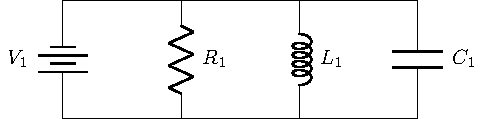
\includegraphics[width=0.7\linewidth]{./LaTex_Tikz/circuitikz.pdf}
	\end{figure}
	\blfootnote{circuitikz -- \url{https://ctan.org/pkg/circuitikz?lang=en
	}}
\end{frame}

\section{How to get started}
\begin{frame}
	asdf
\end{frame}

\end{document}
